\section{Triển khai giao diện quản trị}

Giao diện quản trị của hệ thống Safe Zone được triển khai dưới dạng Ứng dụng Trang Đơn (Single Page Application - SPA) nhằm cung cấp trải nghiệm mượt mà, hạn chế tối đa độ trễ phản hồi khi tương tác với khối lượng dữ liệu giám sát lớn. 

Kiến trúc triển khai mặt trước (Frontend) tuân thủ mô hình tách biệt hoàn toàn giữa Tầng Hiển thị (View Layer) và Tầng Quản lý Trạng thái (State Management):

\begin{figure}[H]
    \centering
    \begin{tikzpicture}[
        node distance=2.2cm,
        box/.style={rectangle, draw=gray!60, rounded corners=4pt, minimum width=2.8cm, minimum height=0.8cm, align=center, fill=blue!5, font=\sffamily\small},
        db/.style={cylinder, draw=gray!60, shape border rotate=90, aspect=0.25, minimum width=2cm, minimum height=1.2cm, align=center, fill=purple!5, font=\sffamily\small},
        biarrow/.style={<->, >=Stealth, thick, draw=gray!80}
    ]
        % Nodes
        \node[box] (ui) {React Components\\(Tailwind CSS)};
        \node[box, below=1cm of ui, fill=green!5] (swr) {SWR State\\(Client Cache)};
        \node[box, right=2cm of swr, fill=cyan!5] (api) {core-api\\(REST Endpoints)};
        \node[db, right=2cm of api] (db) {SQLite / Redis\\(Storage)};

        % Connections
        \draw[biarrow] (ui) -- (swr) node[midway, right, font=\sffamily\scriptsize] {Hooks (useSWR)};
        \draw[biarrow] (swr) -- (api) node[midway, above, font=\sffamily\scriptsize] {HTTP/JSON};
        \draw[biarrow] (api) -- (db) node[midway, above, font=\sffamily\scriptsize] {Query};
    \end{tikzpicture}
    \caption{Luồng dữ liệu và quản lý trạng thái của Giao diện Quản trị}
    \label{fig:ui_data_flow}
\end{figure}

Các kỹ thuật triển khai cốt lõi bao gồm:
\begin{itemize}
    \item \textbf{Đồng bộ trạng thái từ xa (Remote State Cache):} Hệ thống sử dụng thư viện \texttt{SWR} để quản lý trạng thái dữ liệu lấy từ API. Dữ liệu cấu hình, danh sách chặn lọc và số liệu giám sát được lưu trữ an toàn trong bộ nhớ đệm của trình duyệt. Giao diện luôn được hiển thị lập tức từ bộ đệm, song song với việc gọi API ngầm để xác thực lại tính mới của dữ liệu (Stale-while-revalidate), đảm bảo quản trị viên không bị gián đoạn bởi các màn hình chờ tải (Loading Spinners).
    \item \textbf{Trực quan hóa dữ liệu theo thời gian thực:} Tích hợp động cơ vẽ biểu đồ \texttt{Recharts} để thống kê lưu lượng DNS (Telemetry). Dữ liệu được tổng hợp (aggregate) và phân trang trực tiếp từ bộ đệm của \texttt{core-api}, giúp biểu đồ duy trì tốc độ khung hình (FPS) ổn định ngay cả khi hiển thị phân tích của hàng ngàn sự kiện truy vấn cùng lúc.
    \item \textbf{Tối ưu hóa tác vụ mạng (Network Optimization):} Xây dựng hệ thống form tương tác (ví dụ: công cụ cấu hình danh sách đen/trắng, công cụ phân tích rủi ro tên miền độc lập) được bọc trong các Hook bất đồng bộ, tự động xử lý thử lại khi lỗi mạng (network retry) và triệt tiêu các lệnh gọi trùng lặp (debounce) để giảm thiểu áp lực tải cho Backend.
\end{itemize}

Kết quả thực tế sau khi triển khai hệ thống giao diện:

\begin{figure}[H]
    \centering
    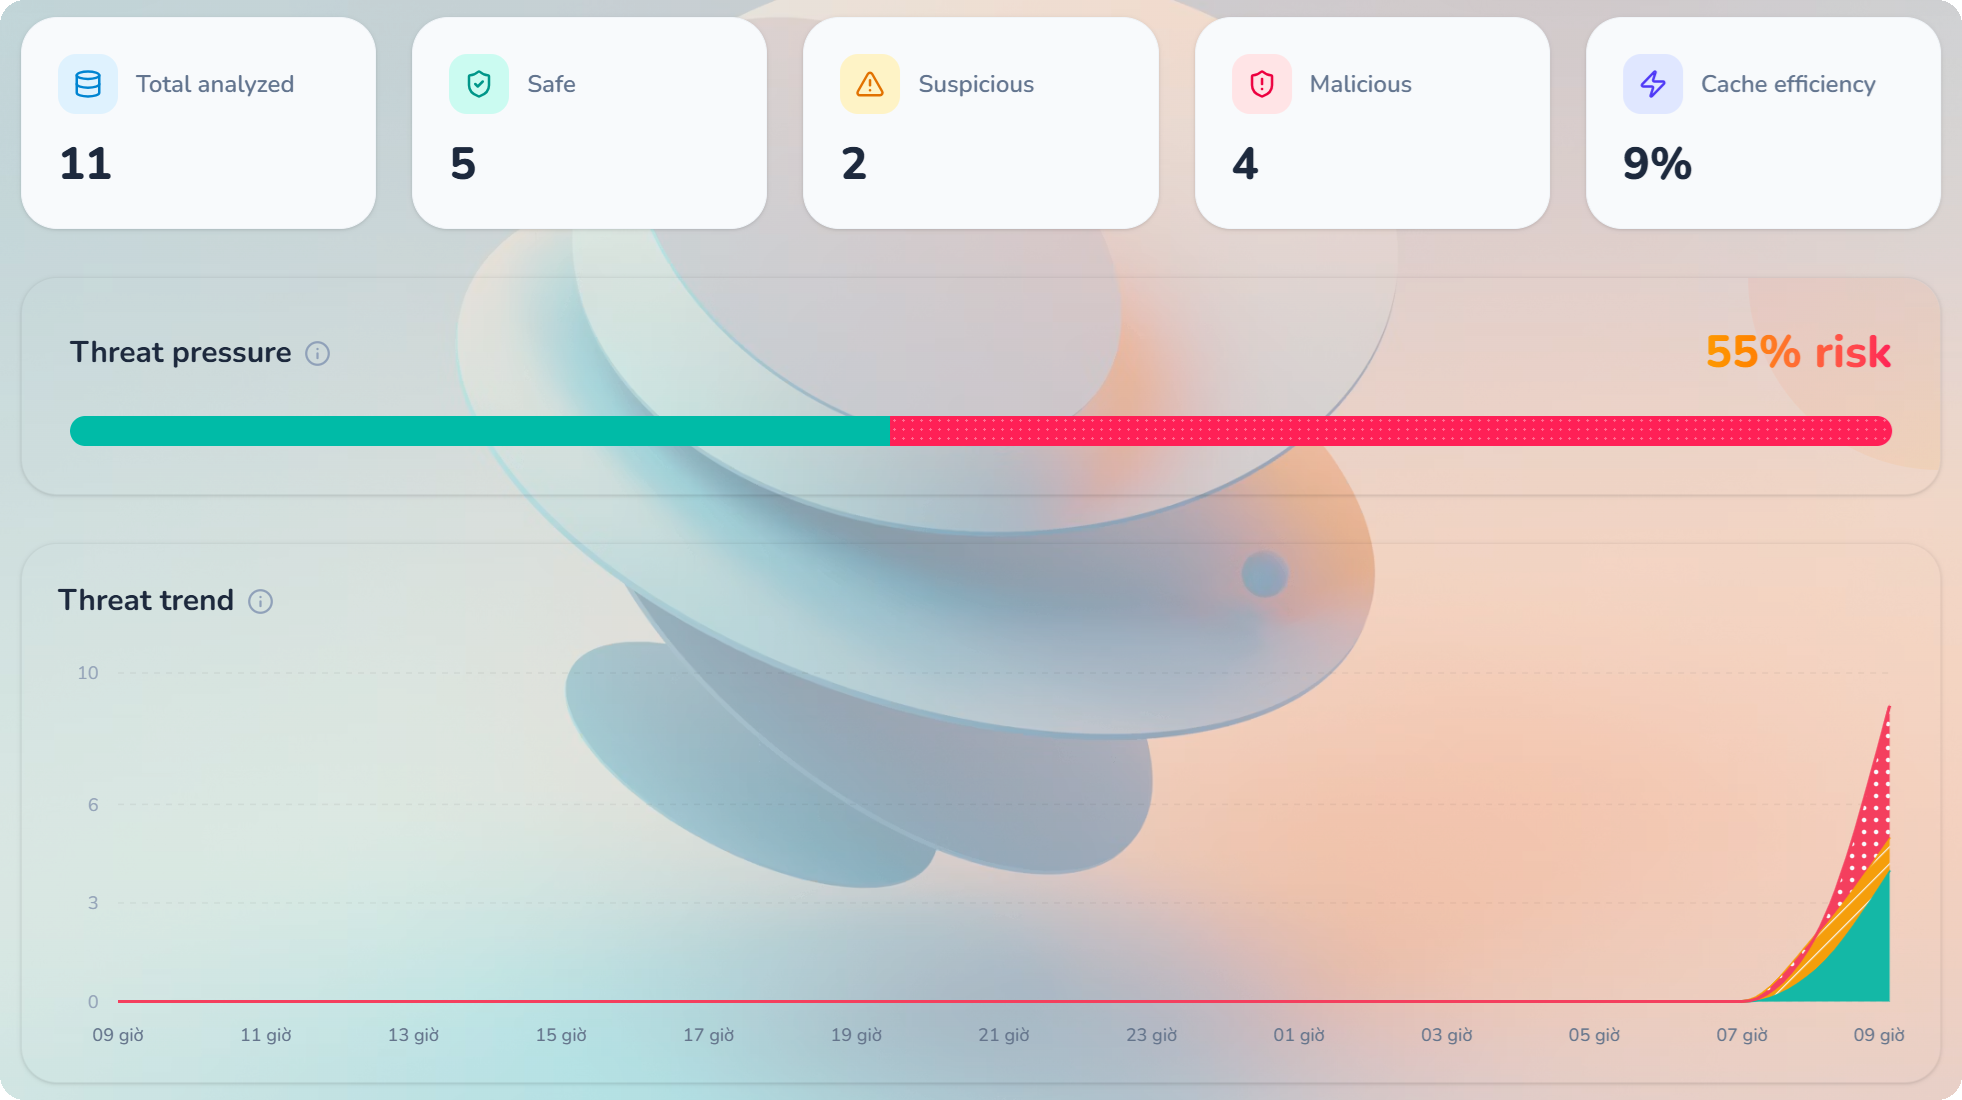
\includegraphics[width=0.9\textwidth]{img/ui_telemetry_1.png} \\
    \vspace{0.5cm}
    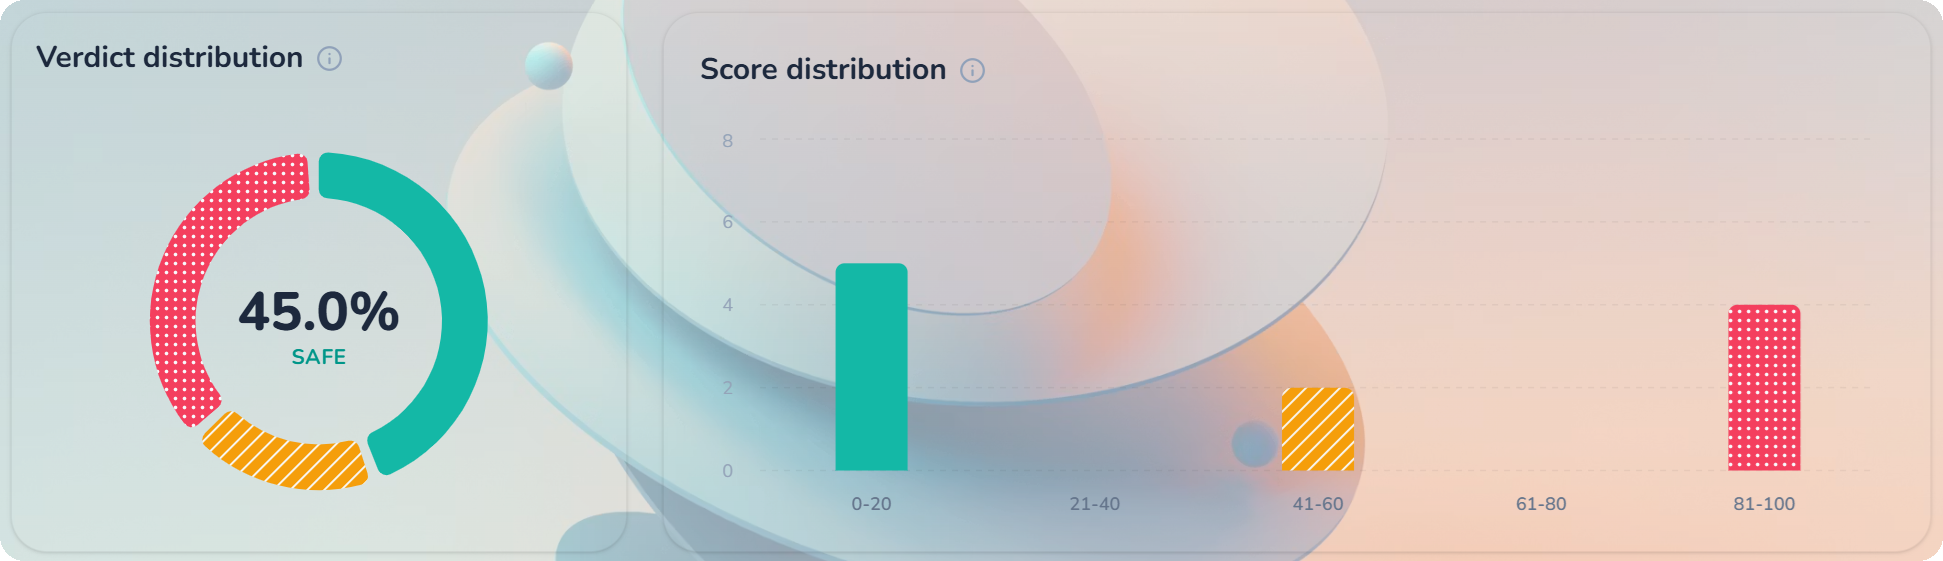
\includegraphics[width=0.9\textwidth]{img/ui_telemetry_2.png}
    \caption{Giao diện Bảng điều khiển (Telemetry) hiển thị thống kê truy vấn và phân phối rủi ro}
    \label{fig:ui_telemetry}
\end{figure}

Bảng điều khiển (Telemetry) đóng vai trò giám sát trung tâm (Hình \ref{fig:ui_telemetry}). Các biểu đồ động trực quan hóa tần suất truy vấn, tỷ lệ phân giải thành công và hiệu suất bộ nhớ đệm giúp quản trị viên đánh giá nhanh mức độ đe dọa (Threat Pressure) trong hệ thống mạng.

\begin{figure}[H]
    \centering
    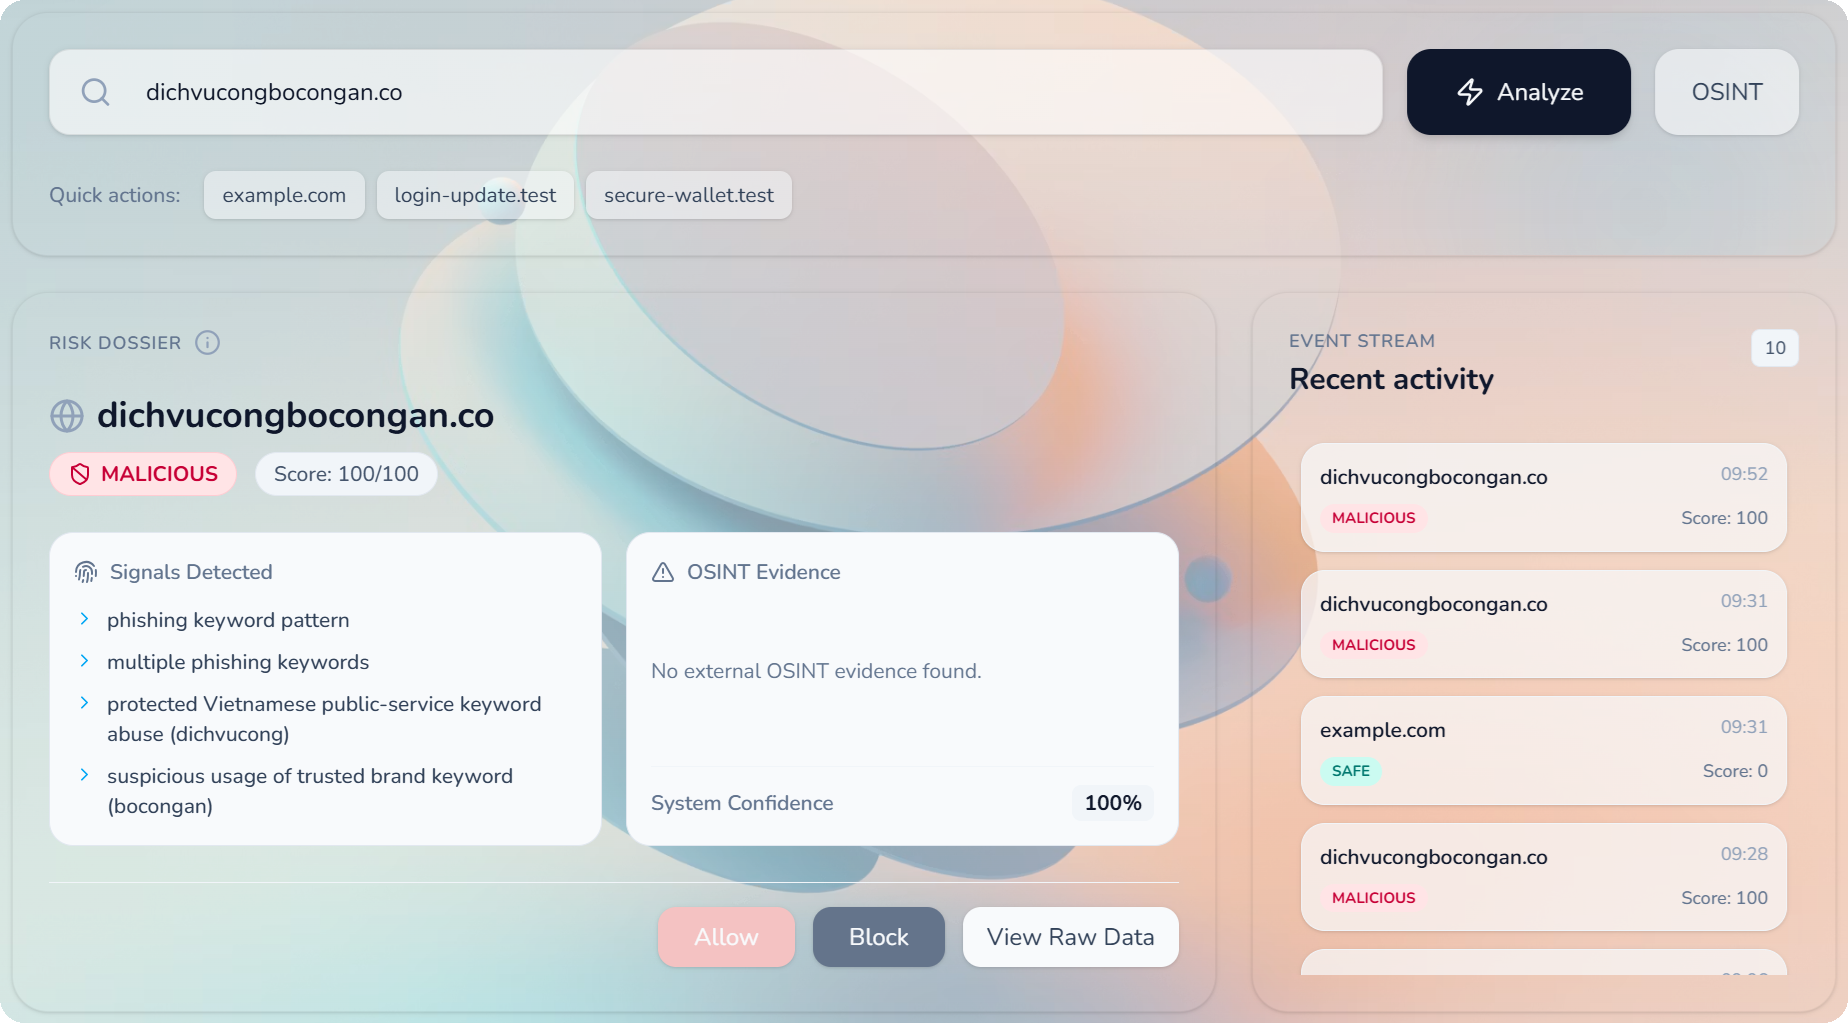
\includegraphics[width=0.9\textwidth]{img/ui_analysis_1.png} \\
    \vspace{0.5cm}
    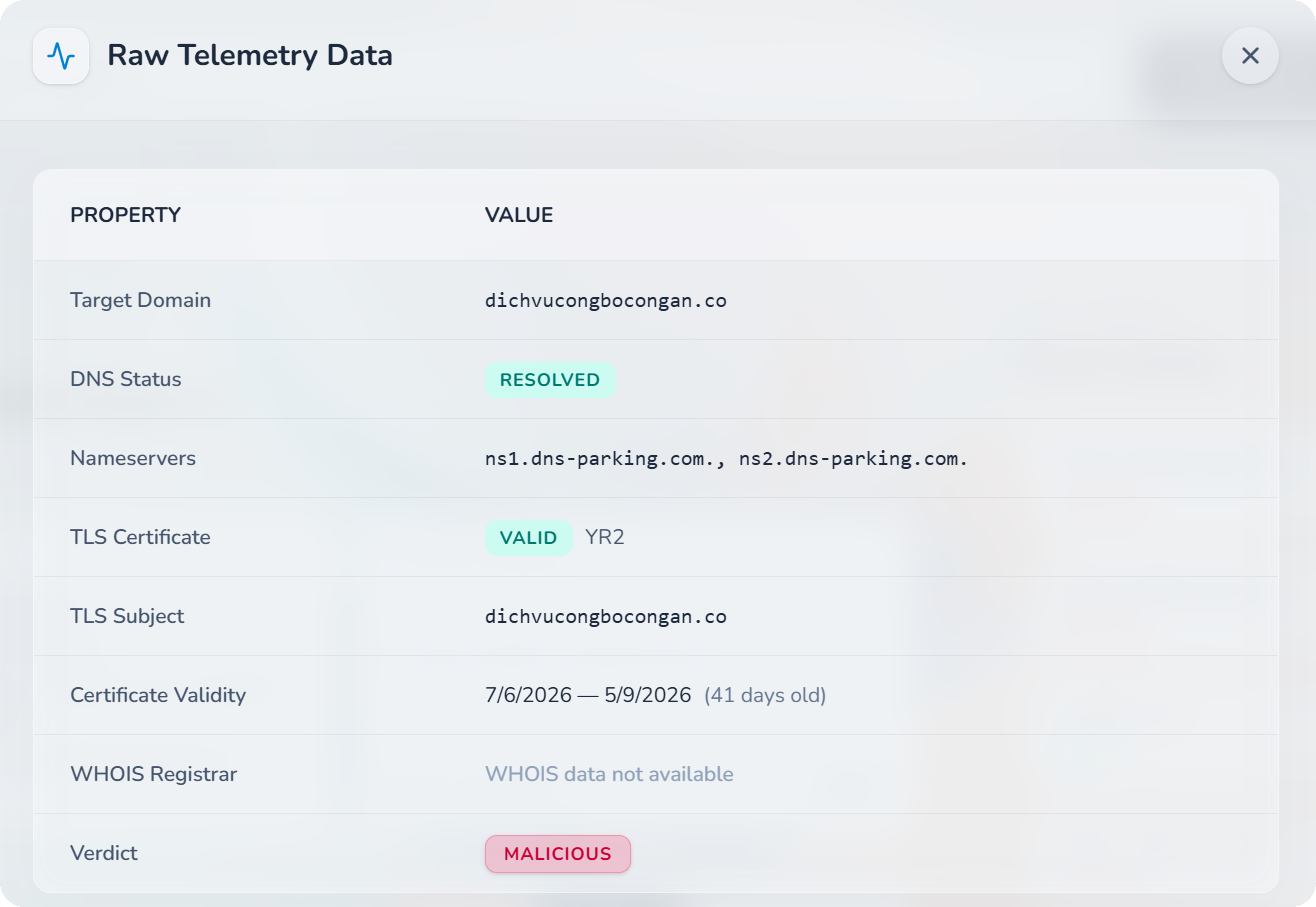
\includegraphics[width=0.9\textwidth]{img/ui_analysis_2.png}
    \caption{Giao diện Phân tích rủi ro tên miền động (Domain Analysis)}
    \label{fig:ui_analysis}
\end{figure}

Giao diện Phân tích (Domain Analysis) cung cấp khả năng kiểm tra sâu một tên miền bất kỳ (Hình \ref{fig:ui_analysis}). Việc bóc tách chi tiết các đặc trưng ngữ vựng (Lexical Features) kết hợp với kết quả suy luận AI mang lại tính minh bạch, giúp người quản trị dễ dàng xác minh tính chính xác của hệ thống.

\begin{figure}[H]
    \centering
    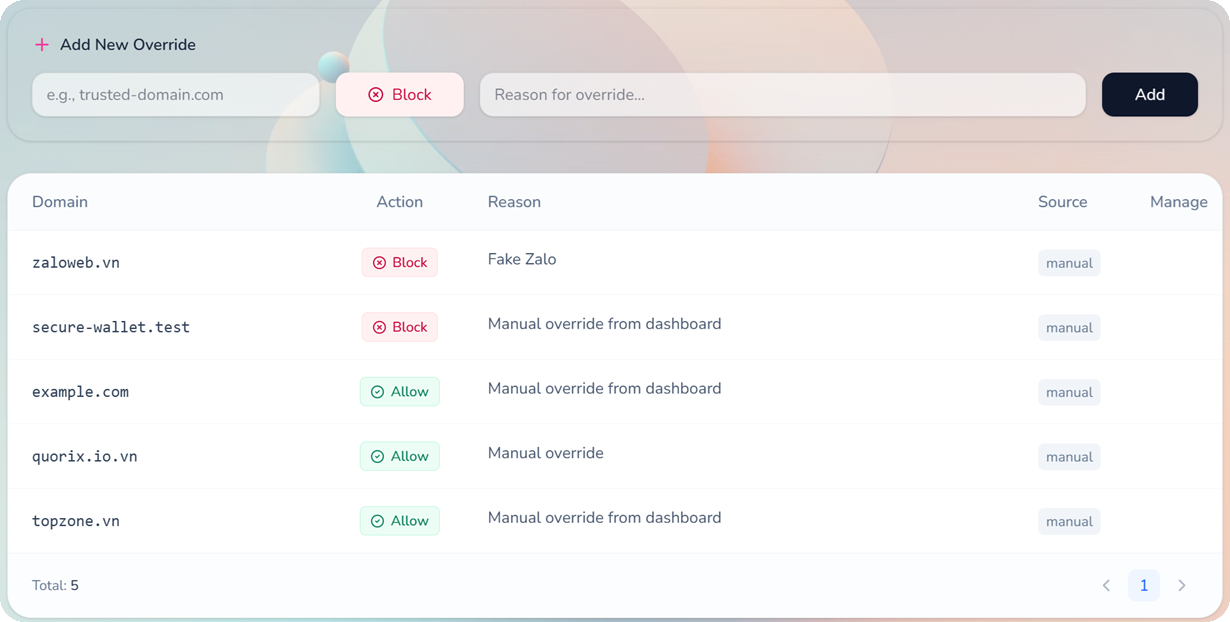
\includegraphics[width=0.9\textwidth]{img/ui_overrides.png} 
    \caption{Giao diện Quản lý danh sách cấu hình ngoại lệ (Overrides)}
    \label{fig:ui_overrides}
\end{figure}

Giao diện Quản lý ngoại lệ (Overrides) là thiết yếu để kiểm soát luồng phân giải (Hình \ref{fig:ui_overrides}). Việc lập Danh sách trắng (Whitelist) và Danh sách đen (Blacklist) giúp giảm cảnh báo nhầm (False Positive) và chủ động chặn đứng tức thời các mối đe dọa tại tầng DNS Resolver.
